\chapter{Results}

I analysed three daily networks, these are refererred to below as \#1, \#2, and \#3. Each network is aggregated for ten hours starting at 8~a.m. and lasting until 6~p.m. I chose the 20.08.2016, 22.08.2016, and 24.08.2016, because at this point in time the hive also contained tagged foragers (older bees). At the same time young bees were added to the colony (see table~\ref{tab:networks} for details). The age distribution for each network is shown in figure~\ref{fig:ages}.

[TODO: PLOT How many nodes in the network stay the same over 3 timesteps? (will be going next step, same, new ones)]

\begin{table}
\centering
\begin{tabular}{ccccccc}
\toprule
{} & 20.08.16 & 21.08.16 & 22.08.16 & 23.08.16 & 24.08.16 \\
\midrule
Network ID & \#1 & - & \#2 & - & \#3 & \\
Number of added bees & 0 & 0 & 110 & 60 & 0 \\
Time added & - & - & 2~p.m. & 6~p.m. & - \\
\bottomrule
\end{tabular}
\caption[TODO]{Overview about networks and number of added bees.}
\label{tab:networks}
\end{table}

\begin{figure}[htb]
	\centering
	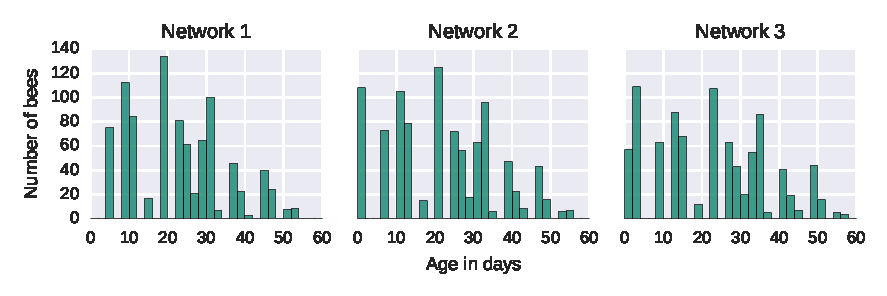
\includegraphics[width=1.0\textwidth]{Figures/ages}
	\caption[Age distribution per network]{Age distribution per network: The width of a bar corresponds to two days.}
	\label{fig:ages}
\end{figure}

\section{Network type and properties}
 
\subsection{Global Structure - Network Level}
Each network consists of one giant component. Table~\ref{tab:stats} summarizes basic network properties number of nodes, number of links, density, diameter, average shortest path length, global clustering coefficient, average degree, and average strength.\\

TODO: high density, small diameter, very short average path length, high clustering coefficient, high strength and degree, compared to what? random graph\\

TODO: calc network centralisation and add to table\\
TODO: PLOT degree and strength distribution\\
TODO: PLOT edge weight distribution\\

\begin{table}
\centering
\begin{tabular}{lcccccccc}
\toprule
{} &  $N$ &   $L$ &  $D$ &  $\langle d_{\texttt{max}} \rangle$ &  $\langle d \rangle$ &   $C_\Delta$ &  $\langle k \rangle$ &  $\langle s \rangle$ \\
\midrule
\#1 &    922 &  291179 &     0.69 &         3 &              1.32 &  0.79 &      631.62 &      5680.17 \\
\#2 &    978 &  256066 &     0.54 &         3 &              1.46 &  0.72 &      523.65 &      3977.94 \\
\#3 &    922 &  259421 &     0.61 &         3 &              1.39 &  0.75 &      562.74 &      4205.99 \\
\bottomrule
\end{tabular}
\caption[Global network properties]{Global network properties}
\label{tab:stats}
\end{table}

\subsection{Local Structure - Node Level}

[TODO: PLOT closeness, betweenness, local clustering coefficient, eigenvector centrality, weighted and unweighted]

\subsection{Network type}

[TODO: compare to random graph]\\
degree distribution random poisson or binominal, not random power law\\
giant component, connectedness\\
average path length and diameter very small, small world phenomenon\\
higher clustering coefficient than in random\\

\section{Network Metrics in Relation to Age of Bees}

[TODO: all plot in relation to age]

\section{Community Detection}

TODO: if time: show that communities are robust in terms of ilen and radius\\
TODO: age: müsste man eigentlich nochmal gegen ein randomisiertes Modell testen. Alter randomisieren\\
TODO: plots der Communities 2community x 3Netzwerke je 4 Kameras\\

Using the leading eigenvector community detection algorithm revealed in all three networks two communities with about the same number of nodes. The exact number of community members is shown in table~\ref{tab:networks}. The first community contains the queen and bees who are on average younger than the second community. The age difference for \#1 is $8.4$ days, for \#2 $10.9$ days, and for \#3 $14.4$ days on average. The age distribution for each community and network is depicted in figure~\ref{fig:ageDistribution}.

A two sample Kolmogorov–Smirnov test showed, that for each network, the age distributions are significantly different ($p=1.7e^{-32} \pm2.9e^{-32}$).

\begin{table}
\centering
\begin{tabular}{ccrrr}
	\toprule
	{}  & Number of members & Proportion & Age & SD\\
	\midrule 
	\#1  & 488     & 52.93\% & $25.15$ & $\pm19.49$ \\
	             & $434^*$ & 47.07\% & $16.81$ & $\pm17.91$ \\
	\midrule   							
	\#2  & $503^*$ & 51.43\% & $15.44$ & $\pm19.54$ \\
	             & 475     & 48.57\% & $26.37$ & $\pm18.01$ \\
	\midrule  
	\#3  & 537     & 58.24\% & $27.26$ & $\pm17.84$ \\
	             & $385^*$ & 41.76\% & $12.85$ & $\pm20.24$ \\
	\bottomrule
\end{tabular}
\caption[Overview about communities]{Overview about communities per network: Communities marked with * contain the queen.}
\label{tab:communities}
\end{table}

\begin{figure}[htb]
	\centering
	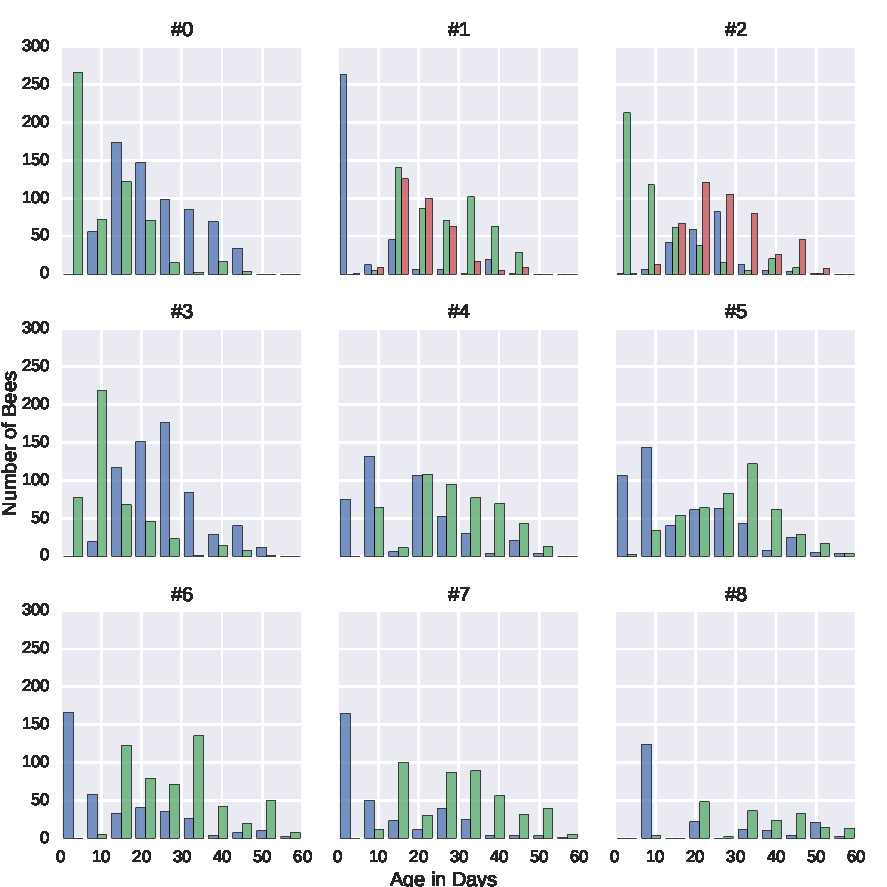
\includegraphics[width=1.0\textwidth]{Figures/ageDistribution}
	\caption[Age distribution for each community and network] {Age distribution for each community and network: The \emph{blue} bar is the community containing the queen. The queens age is not included in the statistic. The \emph{green} bars coresspond to the second community, containing older bees.}
	\label{fig:ageDistribution}
\end{figure}


The younger community containig spends most time in the center of the comb. The older group is situated on the outer parts, this is the same for all 3 networks. This suggest stable communities in termns of age and spatial distribution.

\begin{figure}[b]
	\centering
	\begin{subfigure}[b]{1.0\textwidth}
		\centering
		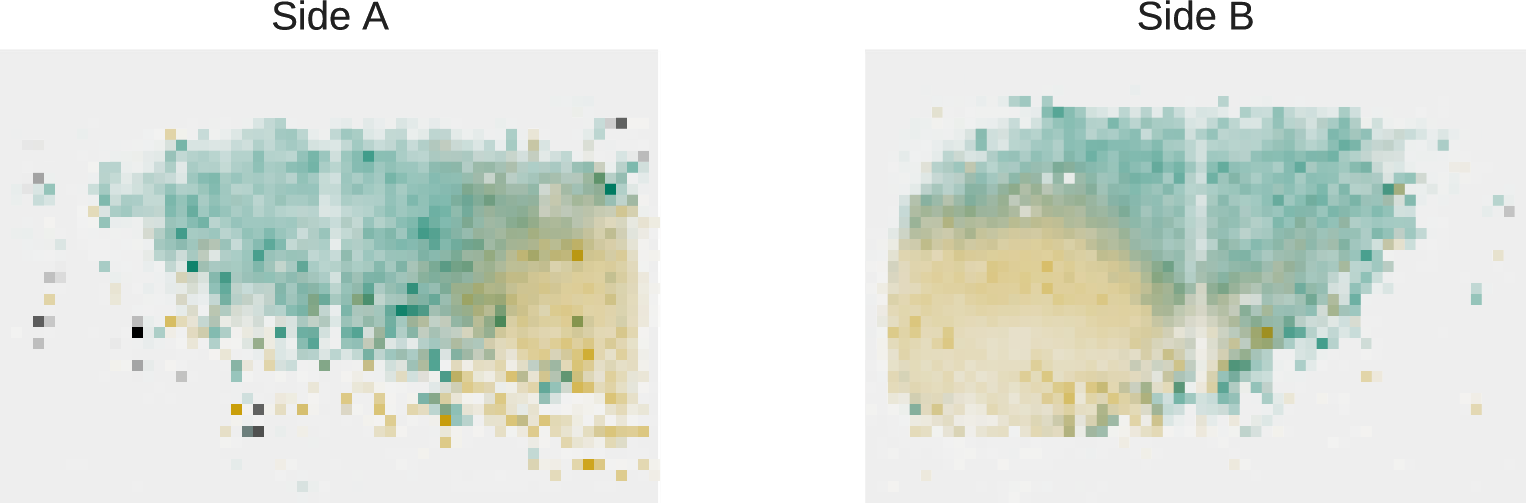
\includegraphics[width=\textwidth]{Figures/network1}
		\caption[Network 1]{Network 1}
		\label{fig:n1}
		\vspace*{5mm}
	\end{subfigure}
	%\vspace{1cm} 
	\begin{subfigure}[b]{1.0\textwidth}
		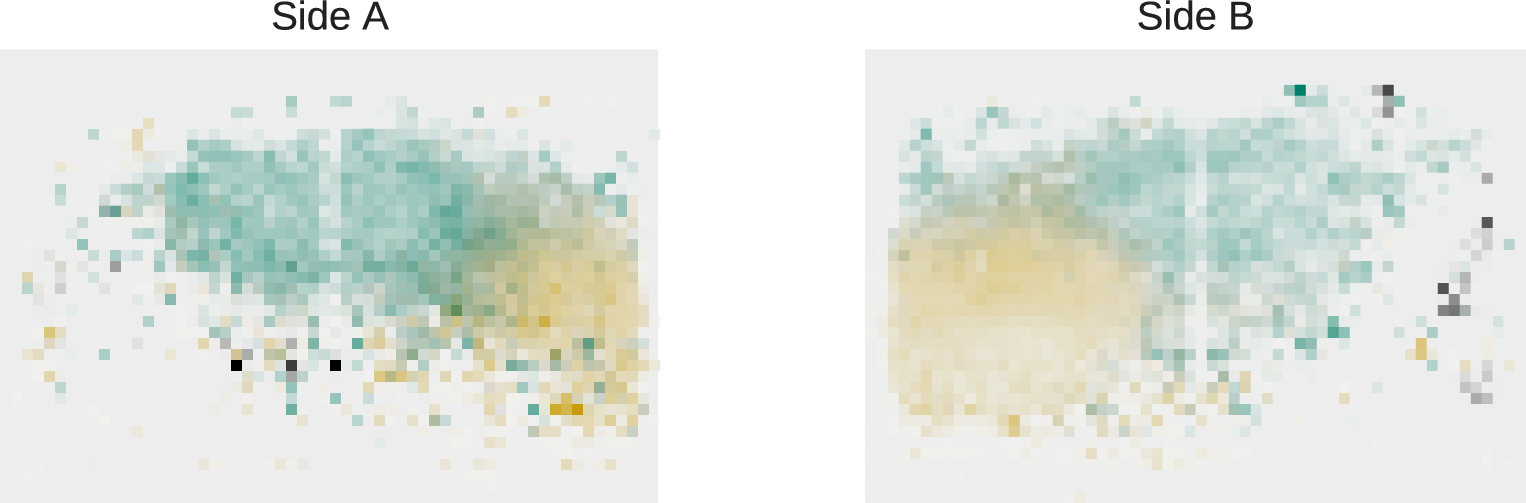
\includegraphics[width=\textwidth]{Figures/network2}
		\caption[Network 2]{Network 2}
		\label{fig:n2}
		\vspace*{5mm}
	\end{subfigure}
	%\vspace{1cm} 
	\begin{subfigure}[b]{1.0\textwidth}
		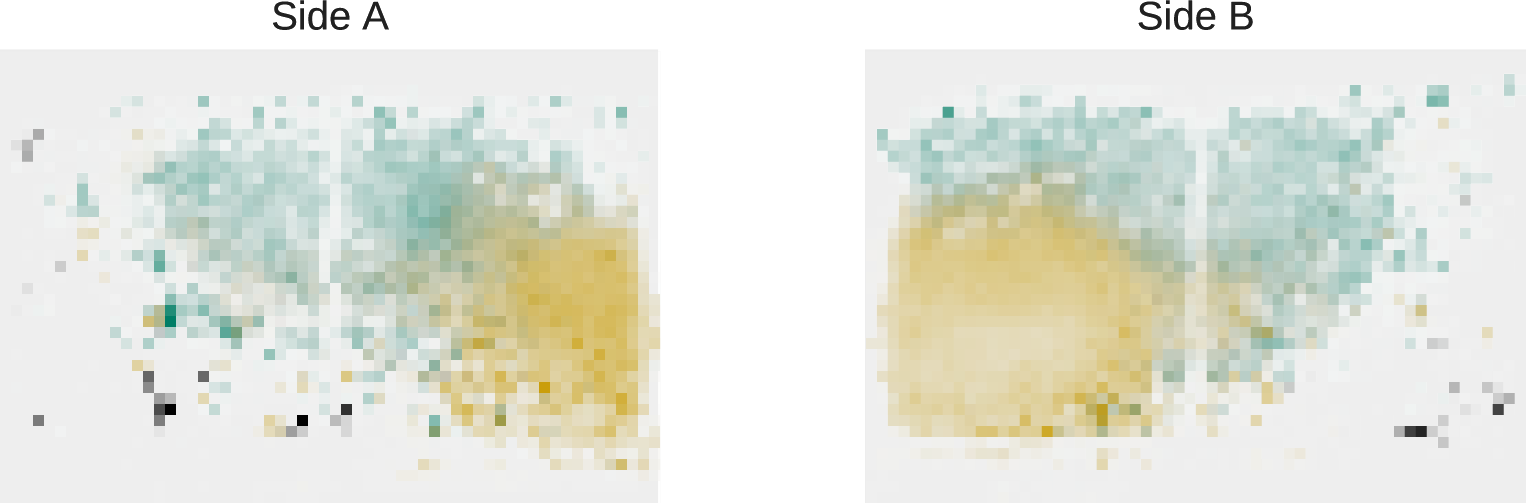
\includegraphics[width=\textwidth]{Figures/network3}
		\caption[Network 3]{Network 3}
		\label{fig:n3}
	\end{subfigure}
	\caption[Communities per network]{The \emph{green} colour represents the younger community, containing the queen, highlighted in \emph{black}. The \emph{orange} color represents the older community. The hive exit on side A is on the bottom right and on side B on the botom left.}
	\label{fig:communitiesPerNetwork}
\end{figure}


\section{Community members over time}
 The match value between the two communities in succesive time steps are calculated with formular~\ref{eq:match} and presented in figure~\ref{fig:members}. The number of bees changing from community A to community B is higher than the other way around. Which makes sense because bees change their duties while they age. this is a good indicator, but needs further investigation to be quantified.

\begin{figure}[htb]
	\centering
	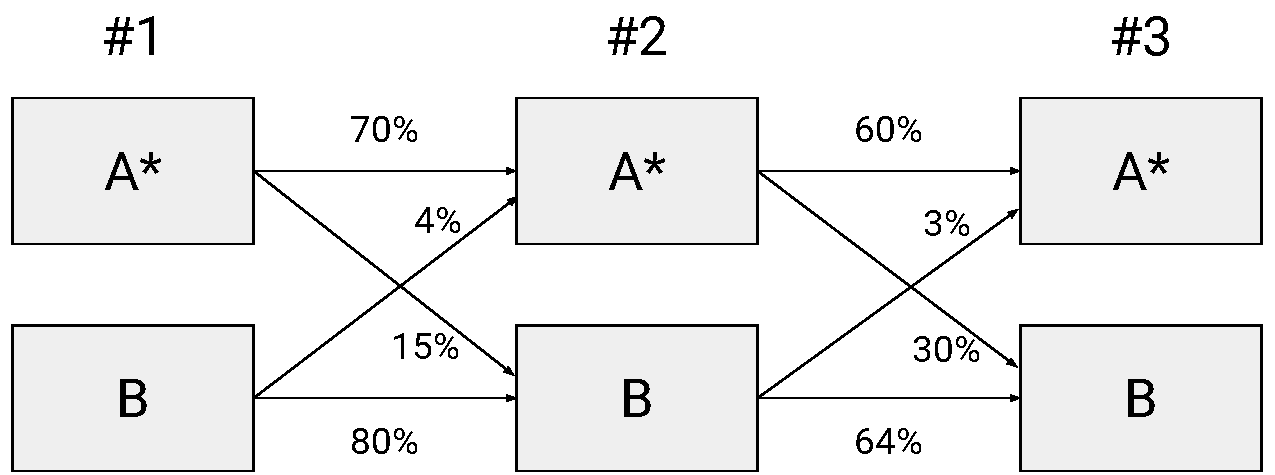
\includegraphics[width=.8\textwidth]{Figures/members}
	\caption[Community Matching]{Community Matching: The numbers indicate the match values. The community marked with * contains the queen and is the younger community.}
	\label{fig:members}
\end{figure}


\section{Summary}
TODO




\begin{figure}[htb]
	\centering
	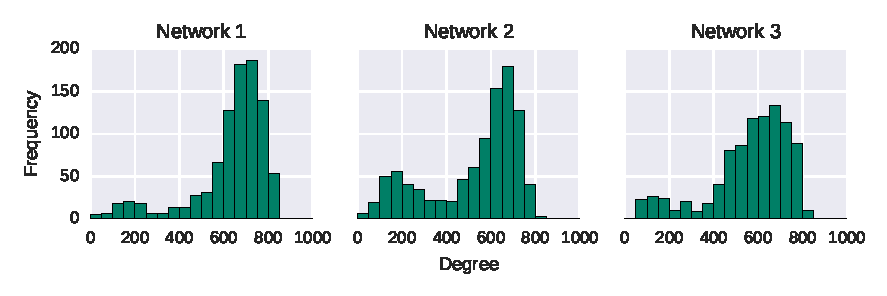
\includegraphics[width=1.0\textwidth]{Figures/stat-degreeDist}
	\caption[Degree Distribution]{Degree Distribution}
	\label{fig:statDegreeDist}
\end{figure}


\begin{figure}[htb]
	\centering
	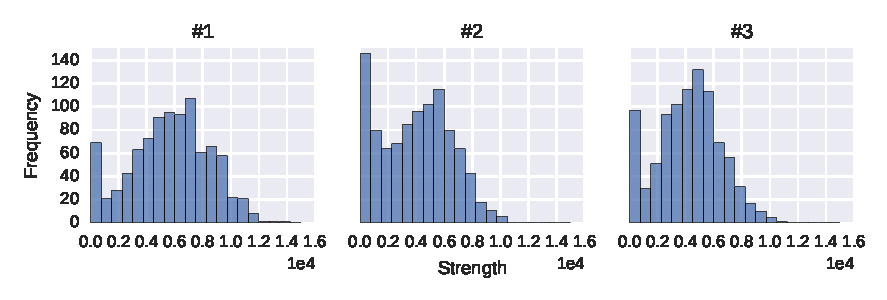
\includegraphics[width=1.0\textwidth]{Figures/stat-strengthDist}
	\caption[Strength Distribution]{Strength Distribution: Weighted Degree Distribution}
	\label{fig:statStrengthDist}
\end{figure}

\begin{figure}[htb]
	\centering
	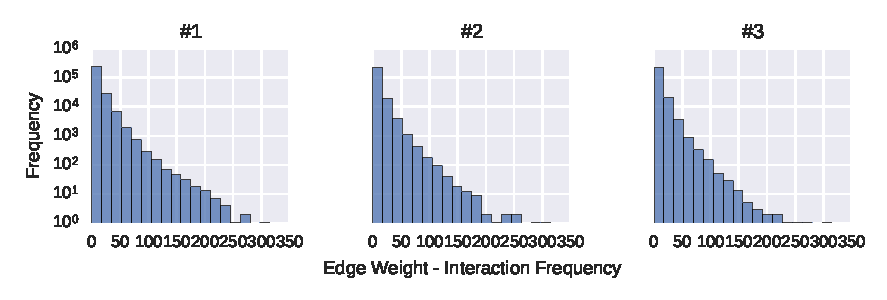
\includegraphics[width=1.0\textwidth]{Figures/stat-edgeWeightDist}
	\caption[Edge Weight Distribution]{Edge Weight Distribution - Edge weight is the contact frequency}
	\label{fig:statEdgeWeightDist}
\end{figure}


\begin{figure}[htb]
	\centering
	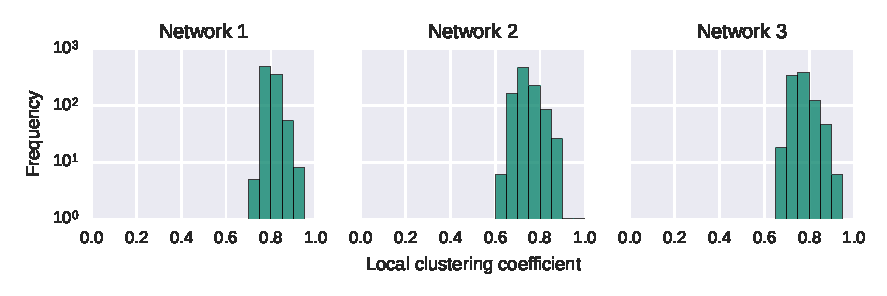
\includegraphics[width=1.0\textwidth]{Figures/stat-lccDist}
	\caption[Local clustering coefficien]{Local clustering coefficien - unweighted}
	\label{fig:lccDist}
\end{figure}


\begin{figure}[htb]
	\centering
	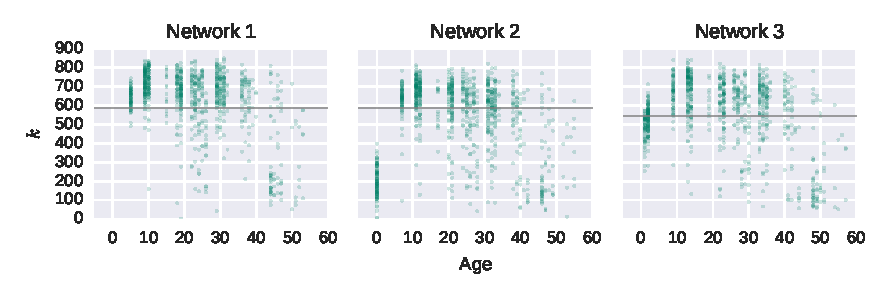
\includegraphics[width=1.0\textwidth]{Figures/stat-degreeAge}
	\caption[Degree VS Age]{Degree versus Age}
	\label{fig:degreeAge}
\end{figure}


\begin{figure}[htb]
	\centering
	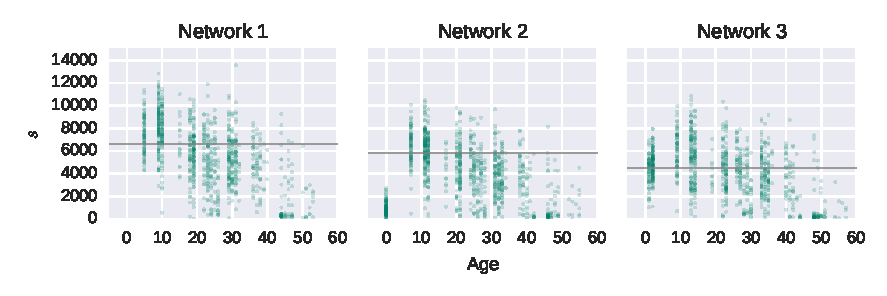
\includegraphics[width=1.0\textwidth]{Figures/stat-strengthAge}
	\caption[Strength Age]{Strength Age}
	\label{fig:strengthAge}
\end{figure}	


\begin{figure}[htb]
	\centering
	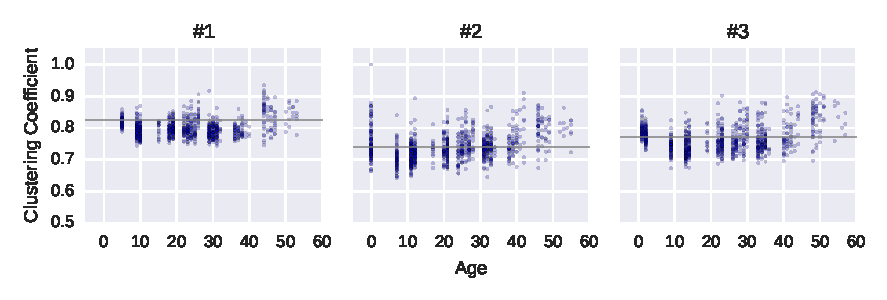
\includegraphics[width=1.0\textwidth]{Figures/stat-ccAge}
	\caption[Local clustering coefficient]{Local clustering coefficient}
	\label{fig:ccAge}
\end{figure}
